%% ma: L12-B13-0018
%% lop: 12
%% chuong: 4
%% bai: 13
%% dang: 12.13.10
%% loai: DS
%% muc: [TH, TH, VD, VDC]
%% dap_an: "SSĐĐ"
%% nguon: "(NBV)-ĐỀ SỐ 6-MỖI NGÀY 1 ĐỀ THI 2025.pdf (D06, MỖI NGÀY 1 ĐỀ - Đề số 6), Phần II Câu 4 (theo Howard Anton, Irl C. Bivens, Calculus AP Edition 11E)"
%% kien_thuc: "Bài 13 (ứng dụng tích phân: thể tích vật thể qua diện tích thiết diện S(x); công); Bài 27 lớp 11 (thể tích khối nón, khối trụ)"
%% trang_thai: cach-ly
%% ly_do: "Đề tự mâu thuẫn, đáp án gốc d) không đúng với dữ kiện. Sau khi bơm sang bể trụ bán kính 4 m cao 0,75 m, thể tích chất lỏng là 12π m3 (không phải 27π m3, là thể tích cả bể nón). Theo lời giải gốc, chất lỏng trong bể nón chiếm các độ sâu x từ 5 đến 9, nhưng khi đó thể tích là π(9^3-5^3)/27 = 604π/27 ≈ 22,4π m3, khác 12π. Lời giải gốc ý a) còn coi chất lỏng là khối nón bán kính đáy 3 m và chiều cao 4 m, không đồng dạng với bể. Nếu lấy đúng thể tích 12π m3 thì chất lỏng chiếm x từ ∛405 ≈ 7,40 đến 9 và công là ρ·π/36·(9^4-405^(4/3)) ≈ 311 000 (Jun), không phải 518014. Gợi ý sửa: đổi chiều cao chất lỏng trong bể trụ thành 604/432 m (≈1,398 m) hoặc đổi dữ kiện thành 'chất lỏng trong bể nón cao 4 m tính từ đáy'; hoặc bỏ ý a), b) và tính công trực tiếp từ độ sâu 5 m đến 9 m"
%% ghi_chu: "Đáp án gốc S S Đ Đ. Ý c) đúng: S(x)=πx²/9 (x là độ sâu tính từ đỉnh nón O). Ý a) sai (27π m3 là thể tích cả bể nón), ý b) sai theo đáp án gốc. Ý d) là chỗ mâu thuẫn. Hình dựng lại theo hình gốc (đỉnh nón O ở trên, trục x hướng xuống)"
\begin{ex}
Một bể hình nón có bán kính đáy là $3$ m và chiều cao là $9$ m đang chứa một lượng chất lỏng. Công thức tính công để hút toàn bộ lượng nước này ra khỏi bể là $W=\displaystyle\int_a^b\rho xS(x)\,\mathrm dx$ (Jun) trong đó $\rho$ $(\text{kg}/\text{m}^3)$ là khối lượng riêng của chất lỏng, $S(x)$ là diện tích mặt cắt (theo Howard Anton, Irl C. Bivens, Calculus AP Edition, 11E, 2016, Wiley).
\begin{center}
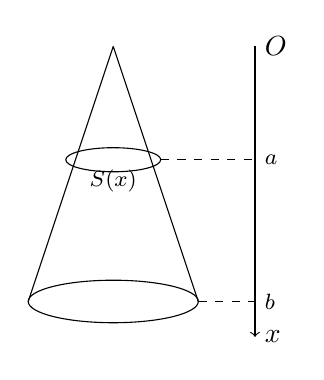
\begin{tikzpicture}[scale=.9]
  \draw (0,3.6)--(-1.2,0) (0,3.6)--(1.2,0);
  \draw (0,0) ellipse (1.2 and .3);
  \draw (0,2) ellipse (.67 and .17);
  \draw[dashed] (.67,2)--(2,2) (1.2,0)--(2,0);
  \draw[->] (2,3.6)--(2,-.5) node[right]{$x$};
  \path (2,3.6) node[right]{$O$} (2,2) node[right,font=\footnotesize]{$a$} (2,0) node[right,font=\footnotesize]{$b$};
  \path (0,2) node[below,font=\footnotesize]{$S(x)$};
\end{tikzpicture}
\end{center}
Từ bể này, người ta hút hết lượng chất lỏng và bơm sang một bể hình trụ có bán kính đáy là $4$ m, khi đó thấy lượng chất lỏng trong bể hình trụ cao $0{,}75$ m.
\choiceTF
{Thể tích chất lỏng là $27\pi$ $(\text{m}^3)$.}
{Chiều cao lượng chất lỏng khi chứa trong bể hình nón là $9$ m.}
{\True Diện tích mặt cắt $S(x)=\dfrac{\pi x^2}{9}$.}
{\True Biết khối lượng riêng của chất lỏng này là $1000\ \text{kg}/\text{m}^3$. Khi đó, công để hút nước từ bể hình nón sang bể hình trụ là $W=518014$ (Jun) (kết quả được làm tròn đến hàng đơn vị của Jun).}
\loigiai{Thể tích chất lỏng bằng thể tích chất lỏng trong bể trụ: $\pi\cdot4^2\cdot0{,}75=12\pi$ $(\text{m}^3)$, nên a) sai ($27\pi$ là thể tích cả bể nón) và chất lỏng không đầy bể nên b) sai. Với $O$ là đỉnh nón, tiết diện ở độ sâu $x$ có bán kính $\dfrac x3$ nên $S(x)=\dfrac{\pi x^2}9$: c) đúng.

Ý d): đáp án gốc tính $W=\displaystyle\int_5^9 1000\cdot\dfrac{\pi x^3}9\,\mathrm dx\approx518\,014$, nhưng lớp chất lỏng giữa $x=5$ và $x=9$ có thể tích $\dfrac{604\pi}{27}\ne12\pi$; theo thể tích $12\pi$ thì cận dưới là $\sqrt[3]{405}$ và $W\approx311\,000$ Jun. Đề mâu thuẫn, xem lý do cách ly.}
\end{ex}
